%\chapter{Microservices}
%\label{ch:microservices}

Upon extracting the real estate data and storing it, it is now necessary to make the data available. This aligns with the goal of creating a cloud application that follows a microservice architecture, where each service is small and focused, so each can be an independent application.

As stated previously, containers are easier to manage when compared to virtual machines, and as they are lightweight, they become an invaluable tool to help us deploy our microservices. However, given that we are bound to have multiple containers, it becomes hard to manage each one independently, as such, we also require a tool to automate the orchestration of all these containers.

Having services broken up into smaller chunks, gives the added benefit of easier failure isolation, as it allows for faster recovery by discovery problems faster. However, by splitting everything into smaller pieces, it becomes a challenge to route traffic between and to services. A way to solve this is through the use of an API Gateway, a special server which acts as the only entry point to the microservices, usually located on the system boundary, encapsulating the internal aspects of the system. One of the drawbacks is that it becomes a single point of failure for the system, as all communication is done through it, but even with this compromise, the benefits outweigh the risks.

One of the characteristics of the microservices architecture is that services are loosely coupled, and one of the ways to achieve this is by assigning a different database to each service. This loose coupling also complicates the communication, however, as microservices are language-neutral, there also language-neutral ways of communicating, such as HTTP via Rest to communicate with the exterior and messages for inter-service communication. 

\subsection{Solution}
\label{ss:backend-solution}

Based on the objectives and proposed solution described previously, we defined what services would be necessary to obtain our application \acrfull{mvp}, and as such the following service definitions were drafted:

\begin{itemize}
    \item \textbf{Estate}: estates (or listings) are considered the main component of the application and as such a microservice to manage it, is required. As such, it is responsible for all information related to the estates (e.g., estate coordinates, price);
    \item \textbf{Parameter}: From the idea of the social functions of the 15-minute city, the Parameter service was born, responsible for dealing with all the information related to points of interest;
    \item \textbf{User}: To classify each house according to each specific user, it was necessary to create a service to manage user information (e.g., personal preferences);
    \item \textbf{Authentication}: To have users, they need to be capable of authenticating and registering themselves within the application; 
    \item \textbf{Metrics}: The relation between the user, estates and parameters (index) is dealt with within the Metrics microservice. It is also used to manage all the metrics associated with each zone;
    \item \textbf{Search}: Since the user needs to search for locations of interest within the application, a service was created to support the search bar.
\end{itemize}

These services in conjunction with the previous storage solutions studied, let to the creation of the architecture presented in Fig. \ref{fig:microservices-overview}.

\begin{figure}
	\centering
	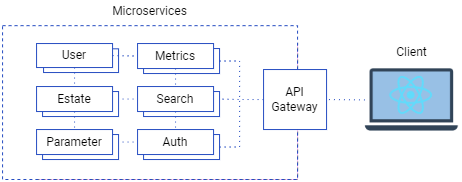
\includegraphics[width=1\textwidth,clip,trim=0 0 0 0]{Chapters/img/backend/ArqOverview_Focused.png}
    \caption[Microservice diagram]{Diagram of available microservices with client requests being funneled through the API Gateway} 
    \label{fig:microservices-overview}
\end{figure}

Each service has its own container, and as the main technology used to implement each service is Java we tried to facilitate the building of Docker images by using \textbf{JIB}~\footnote{See: \url{https://github.com/GoogleContainerTools/jib}}, a tool from Google that builds optimized Docker images without having to depend on a Docker daemon. To deploy them in the \acrshort{k8s}, a Kubernetes service and deployment are also built, with a configuration similar to the one shown in Listing \ref{lst:k8s-deployment}. 

The main takeways from this deployment is how we have organized our kubernetes through the use of namespaces, in this case, all of our backend services are under the namespace \textit{backend}. Followed by the pod configuration each ditactes how many pods will be deployed (number of \textit{replicas}), their names, what docker image to use and from where to pull it, the assigned resources and finally, how to deal with cases of failure (restartPolicy) such as crashes.

\begin{lstlisting}[float,caption={[Microservice Kubernetes deployment configuration]{Example of a \acrshort{k8s} deployment configuration in YAML for a microservice}}, label={lst:k8s-deployment}, captionpos=t]
kind: Deployment
apiVersion: apps/v1
metadata:
  name: be-account-deployment
  namespace: backend
spec:
  replicas: 1
  selector:
    matchLabels:
      app: be-account
  template:
    metadata:
      labels:
        app: be-account
    spec:
      containers:
        - name: be-account
          image: biole/account:latest
          imagePullPolicy: Always
          resources:
            limits:
              memory: "300Mi"
              cpu: "1000m"
          ports:
            - containerPort: 80
      restartPolicy: Always
\end{lstlisting}

In the service configuration, as shown in Listing \ref{lst:k8s-service}, once again we set it up under the backend namespace and configure its type, NodePort, that assigns a static port from a range specified between 30000 and 32767, which makes the service now accessible from outside the cluster. This port can also be manually assigned, as we have done in our configuration. Each service has a port assigned in its spring configuration, for this case its 8083, which is then exposed in \acrshort{k8s} through the port 31003.

\begin{lstlisting}[float, caption={YAML configuration of a Kubernetes service}, label={lst:k8s-service}, captionpos=t]
kind: Service
apiVersion: v1
metadata:
  name: be-account-service
  namespace: backend
spec:
  type: NodePort
  ports:
    - port: 8083
      targetPort: 8080
      protocol: TCP
      nodePort: 31003
  selector:
    app: be-account
\end{lstlisting}

With the increasing number of services, it became difficult to remember and keep track of all existing ports, which was one of the many reasons that led to the implementation of an API Gateway, as seen in Fig. \ref{fig:microservices-overview}. With it, it is now possible to assign URIs to the services, facilitating the access from the frontend as 10.62.73.47:31003 now becomes 10.62.73.47/v1/authentication. Our implementation of an API gateway was done through the use of NGINX~\footnote{\url{https://www.nginx.com/}}, a snippet of the required configuration can be seen in the Listing \ref{lst:nginx-api-gateway}.

It also possible to observe in Fig. \ref{fig:microservices-overview} that the API Gateway acts as a single entry point to the system. Even though the possibility of becoming overloaded with requests exists, the way it simplifies the system overshadows those defects. By having an API Gateway it becomes unnecessary to know the ports of each service, as we can call it through a predefined URI. It also allows us to deal with authentication at this level, this way it is not necessary to verify if the user is authenticated beyond the gateway.

\begin{lstlisting}[float, caption={NGINX API Gateway snippet}, label={lst:nginx-api-gateway}, captionpos=t]
server {
    listen 80;
    server_name 10.62.73.47;

    location /v1/authentication/ {
        proxy_pass http://10.62.73.47:31003;
    }
    ...
}
\end{lstlisting}


\subsubsection{Authentication}

The authentication is supported by \textbf{AWS Cognito}~\footnote{\url{https://aws.amazon.com/cognito/}}, an Amazon platform that provides authentication, authorization, and user management for applications, it allows the user to sign in with credentials or through third party platform such as Facebook and Google. Through the use of Cognito Java \acrshort{api} we managed to create and expose through a Spring Boot \acrshort{api} the following functionalities available at /v1/auth:

\begin{enumerate}
    \item \textbf{login} (POST: /login): authenticate user with the provided credentials;
    \item \textbf{create user} (POST: /create\_user): create a new account by providing an username and an email, a temporary password is sent via email to complete the registration;
    \item \textbf{username lookup} (POST: /username\_lookup): recover the username registered by providing the email used during registration;
    \item \textbf{change password} (POST: /change\_password): alter the provided password by introducing the current password and the new password, the method implementation also accepts as input the type of password change to distinguish between freshly created accounts that have not logged in yet and normal accounts;
    \item \textbf{forgot password} (POST: forgot\_password): if the user forgets his password he can provide the registered username and code will sent to the email associated with the account;
    \item \textbf{reset password} (POST: reset\_password): after the user receives his code for password recovery from the last step, the element can be introduced along with his new password to change it; 
\end{enumerate}

Cognito upon sign-in returns a \acrfull{jwt} which is a JSON encoded representation of a claim(s) that can be transfered between two parties. This claim is digitally signed by the issuer of the token, and the party receiving this token can later use this digital signature to prove the ownership of the claim. This claims are used to provide authentication to the party receiving the token.

\begin{lstlisting}[float, caption={Route with authentication}, label={lst:nginx-api-gateway-auth}, captionpos=t]
location /v1/search/ {
        auth_request /auth/query_auth;
        proxy_pass http://10.62.73.47:31004;
}

location /auth/query_auth {
    proxy_pass http://10.62.73.47/v1/aws/auth/validate-jwt;
    proxy_pass_request_body off;
    proxy_set_header Content-Length "";
    proxy_set_header X-Original-URI $request_uri;
}
\end{lstlisting}

In this application, upon sign in each request includes the token associated with the logged-in user, granting him access to the platform by proving their identity. To validate the claim in every protected route we used the \textit{ngx\_http\_auth\_request\_module} module from NGINX, which implements client authorization based on the result of a subrequest, if the subrequest returns a 2xx response code, the access is allowed. If it returns 401 or 403, the access is denied with the corresponding error. Any other response code is considered an error. This implementation can be seen in the Listing \ref{lst:nginx-api-gateway-auth}, where search performs a subrequest to an endpoint implemented in the authentication microservice.

Since the request originates in Cognito, it also has to be validated with the corresponding information provided from AWS, in this case in the form of a public \acrfull{jwk} located in \textit{https://cognito-idp.{region}.amazonaws.com/{userPoolId}/.well-known/jwks.json.} (\textbf{userPoolId} parameter represents the user directory in Cognito created for this application). With this key it is now possible to verify the signature, as shown in Listing \ref{lst:auth-endpoint}.

\begin{lstlisting}[float, language={Java}, caption={Authentication endpoint}, label={lst:auth-endpoint}, captionpos=t]
@GetMapping("/validate-jwt")
public ResponseEntity<String> validateJWT(@RequestHeader("Authorization") String token) {
    
    String[] tokenSplit = token.split(" ");
    String tokenWithoutBearer = (tokenSplit.length > 1) ? tokenSplit[1] : token;

    DecodedJWT jwt = null;
    try {
        jwt = JWT.decode(tokenWithoutBearer);
    } catch(JWTDecodeException e){
        return ResponseEntity.status(HttpStatus.UNAUTHORIZED).body("Invalid JSON format");
    }

    assert jwt != null;

    JwkProvider provider = new UrlJwkProvider(ENV.JWK_PROVIDER);

    Jwk jwk = null;
    try {
        jwk = provider.get(jwt.getKeyId());
    } catch (JwkException e) {
        return ResponseEntity.status(HttpStatus.INTERNAL_SERVER_ERROR).body("JKW Provider is down");
    }

    assert jwk != null;

    Algorithm algorithm = null;
    try {

        algorithm = Algorithm.RSA256((RSAPublicKey) jwk.getPublicKey(), null);
        algorithm.verify(jwt);
    } catch (InvalidPublicKeyException e) {
        return ResponseEntity.status(HttpStatus.UNAUTHORIZED).body("Invalid token");
    }

    // Check expiration
    if (jwt.getExpiresAt().before(Calendar.getInstance().getTime())) {
        return ResponseEntity.status(HttpStatus.UNAUTHORIZED).body("Expired");
    }

    return ResponseEntity.ok("Authorized");
}
\end{lstlisting}


\subsubsection{User} 
\label{sss:user}

Upon completing his registration and authentication, the user can now start interacting with the platform. As stated previously, the first step is to ask the user to fill his profile information as a way to improve the index performance and tailor it to each user needs. It is split into three different phases as shown in Fig. \ref{fig:profile-stepper} and described in the following list:

\begin{enumerate}[(a)]
    \item Multiple categories that the user must order, through a drag and drop interaction, based on the order of preference;
    \item Targeted at the estate itself, it allows the user to choose the five most important features, for him, in a house;
    \item Selecting the most common way of travel, as to decide how to calculate the radius for the 15-minute city algorithm and choosing what importance to attribute to the previous options.
\end{enumerate}

\begin{figure}[h]
    \centering
    \begin{subfigure}[b]{0.3\textwidth}
        \centering
        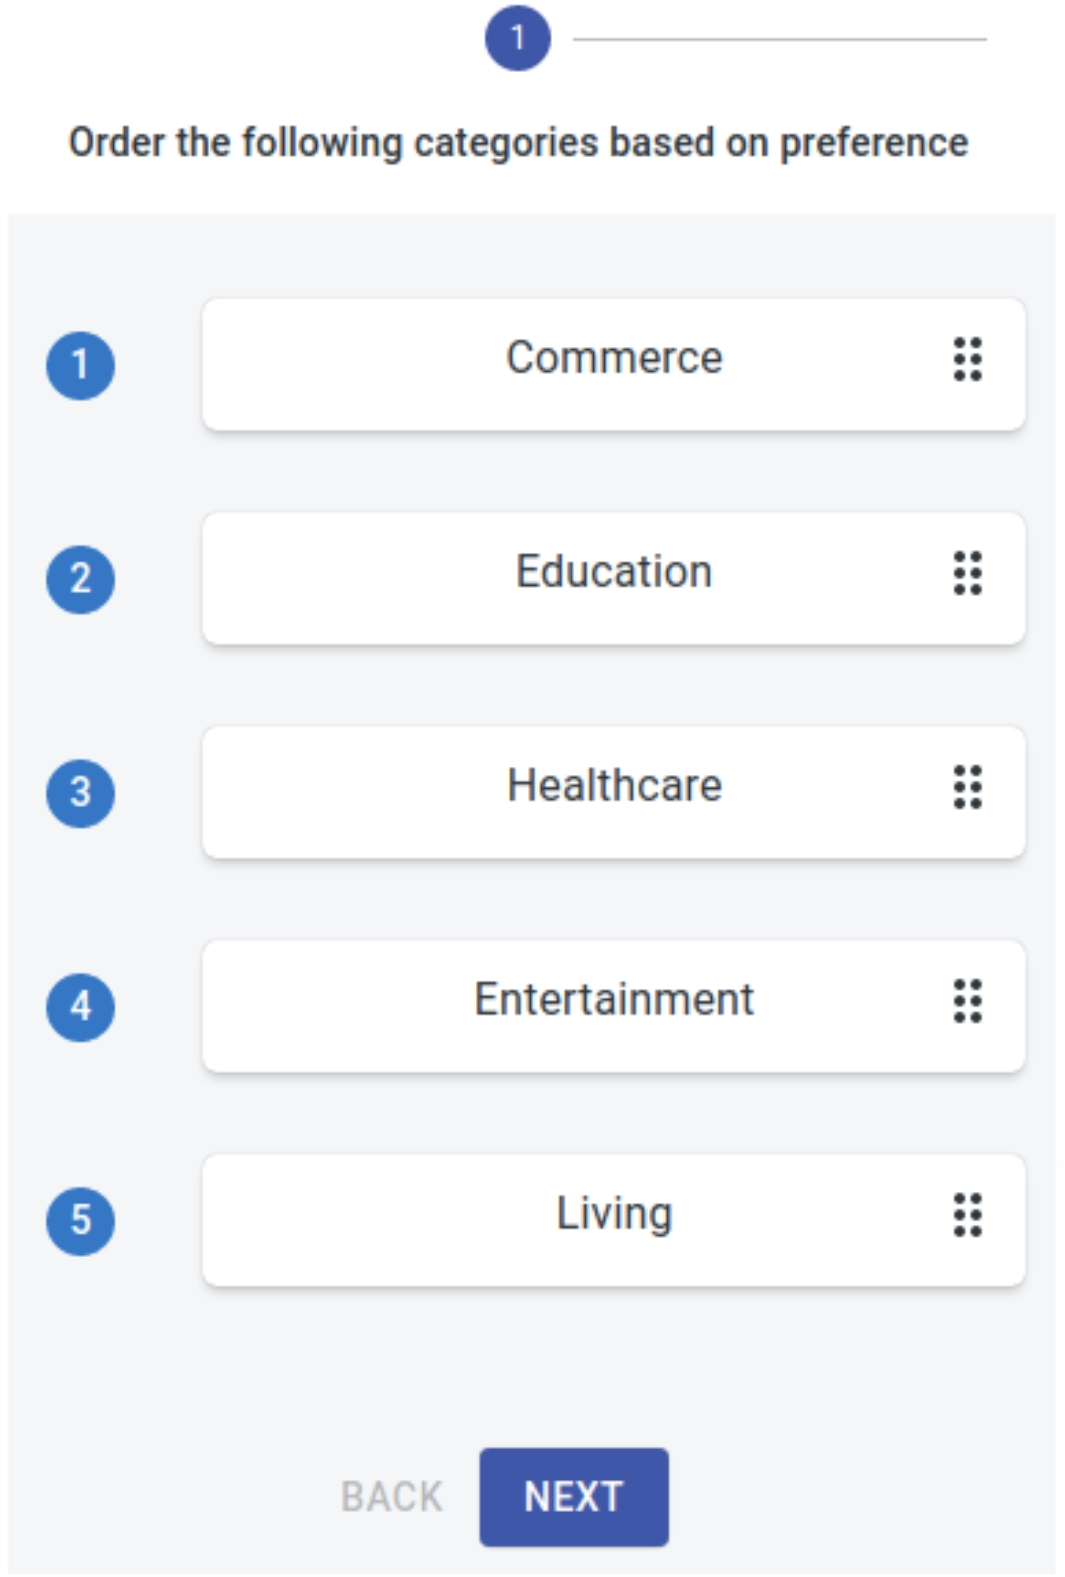
\includegraphics[width=0.85\textwidth]{Chapters/img/backend/ui_stepper_1.png}
        \caption{\centering}
        \label{fig:ui-stepper-1}
    \end{subfigure}
    \hfill
    \begin{subfigure}[b]{0.3\textwidth}
        \centering
        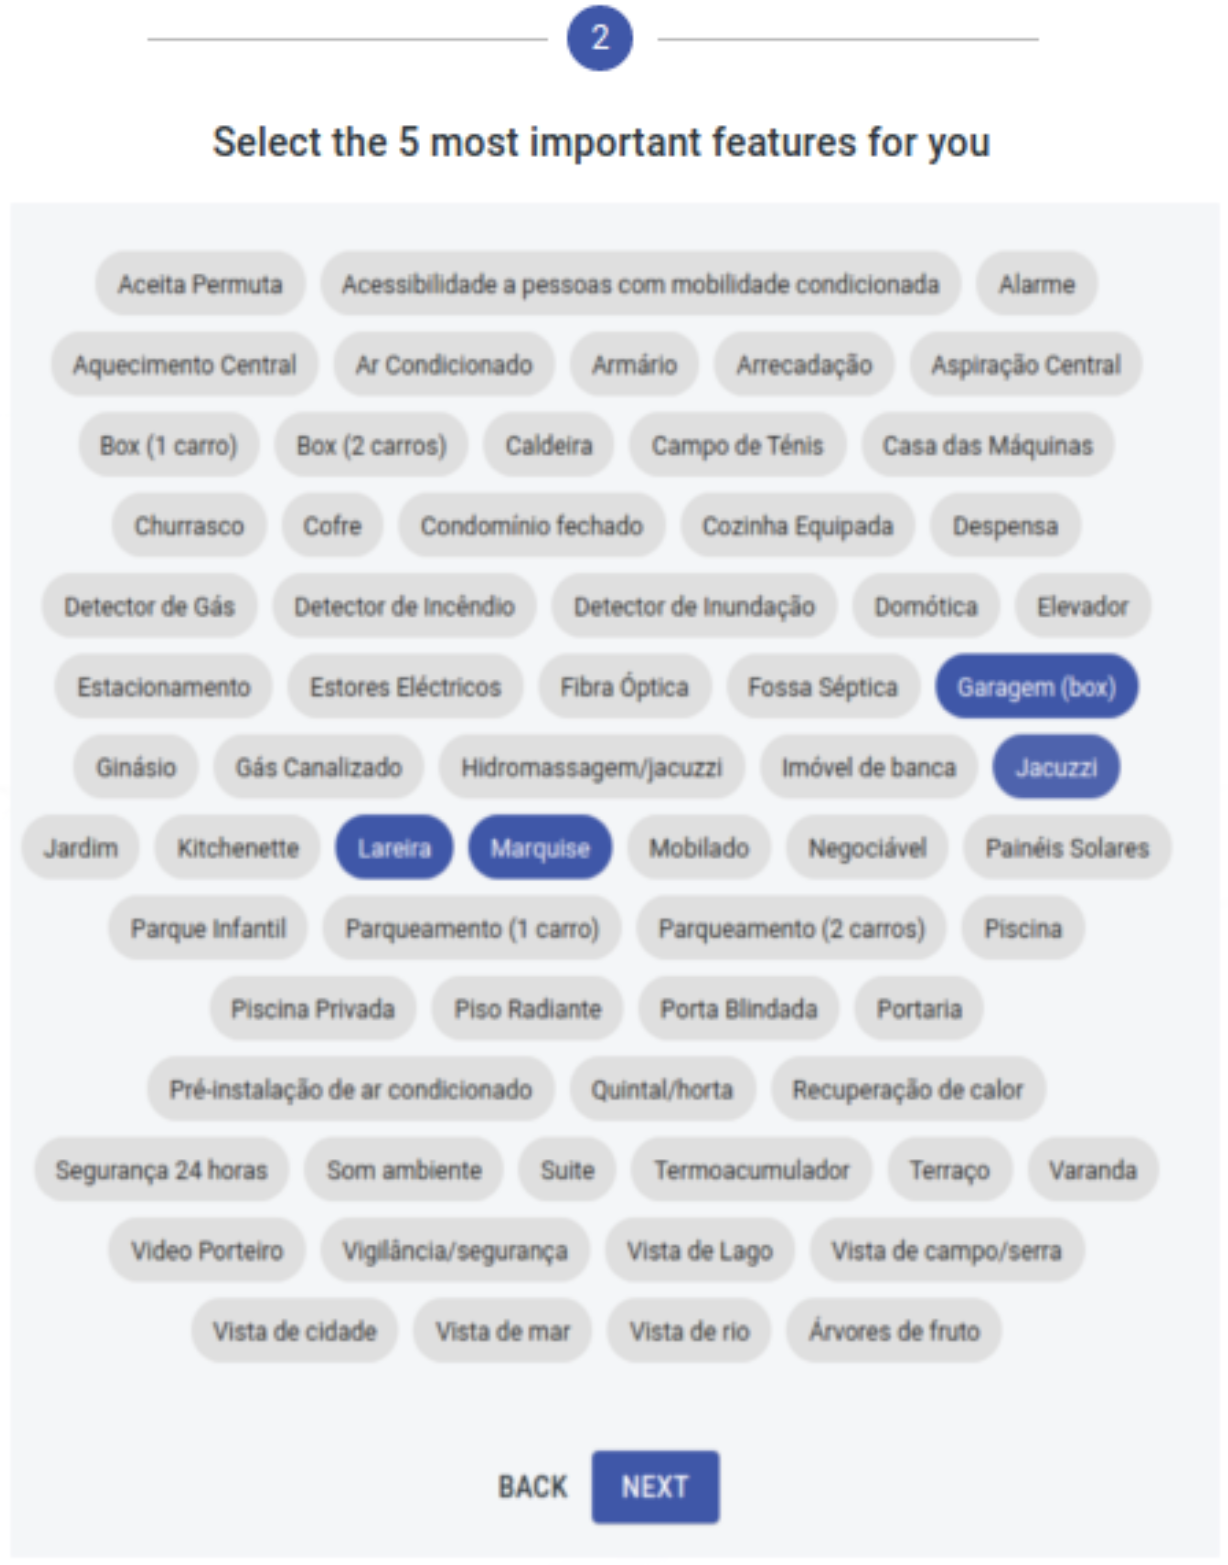
\includegraphics[width=0.99\textwidth]{Chapters/img/backend/ui_stepper_2.png}
        \caption{\centering}
        \label{fig:ui-stepper-2}
    \end{subfigure}
    \hfill
    \begin{subfigure}[b]{0.3\textwidth}
        \centering
        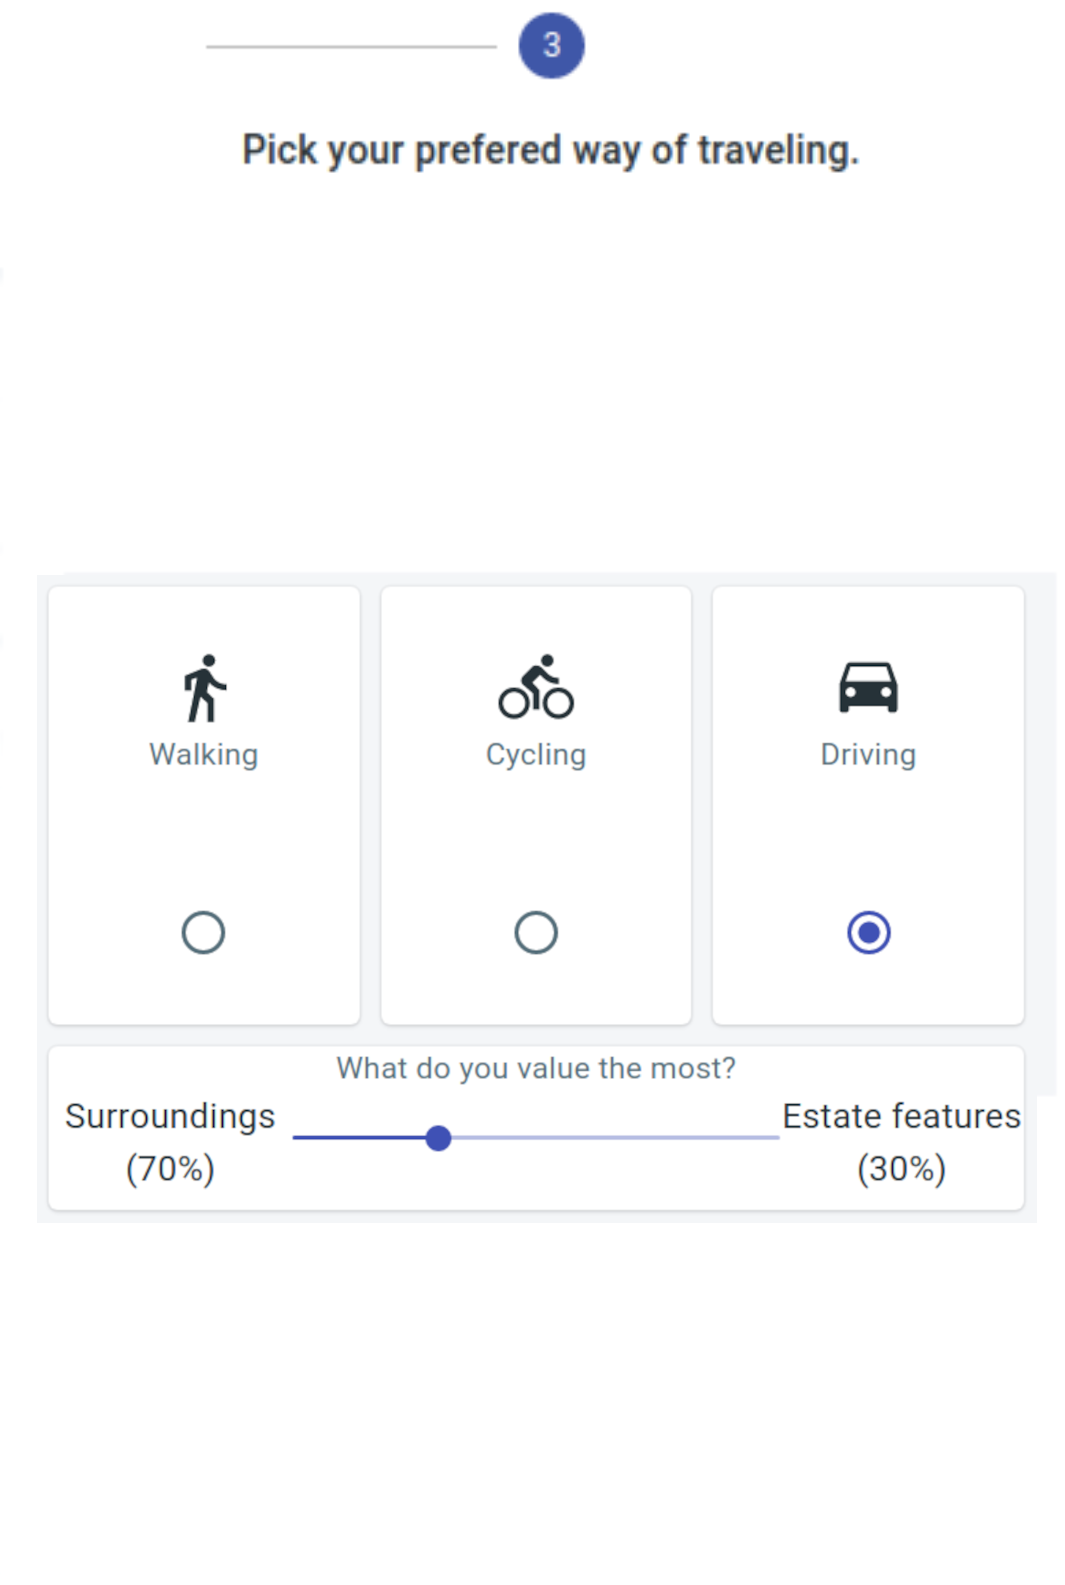
\includegraphics[width=0.85\textwidth]{Chapters/img/backend/ui_stepper_3.png}
        \caption{\centering}
        \label{fig:ui-stepper-3}
    \end{subfigure}
    \caption{Profile creation steps}
    \label{fig:profile-stepper}
\end{figure}

As the authentication credentials were already stored in \acrshort{aws} we have decided to also use another one of their services to store the remainder of user information, which led to the decision of picking DynamoDB a hosted NoSQL database as a storage solution.

\begin{lstlisting}[float, language=Java, caption={[User data model for DynamoDB]{Data model of the User in DynamoDB}}, captionpos=t]
"User": {
    "id": "String",
    "username": "String",
    "ServicePreferences": "List",
    "FeaturePreferences": "Number Set",
    "travelMode": "String"
}
\end{lstlisting}

Personal information was stored according to model shown in Fig. \ref{fig:dynamo-model}, composed of the following elements: 

\begin{enumerate}
    \item An entry identifier of type string, that also acts as a partition key;
    \item An username that ties the information together with Cognito, acting as a foreign key;
    \item the services preferences, stored inside a list that ensures ordering is maintained;
    \item the feature preferences stored in a number set, composed of the identifiers used in the estates database obtain through scraping;
    \item finally, travel mode a string which identifies the preferred travelling mode;
\end{enumerate}

Just like Cognito, the connection to DynamoDB was done through the available AWS SDK for Java, which allowed the creation and management of the database through code. Data access was done with the help of the \textbf{Spring Data}~\footnote{\url{https://spring.io/projects/spring-data}} project, which facilitates application access to data through the use of repositories, which are created with dynamic query derivation from their names (e.g., for SQL with the following java method declaration: Estate findByID(String idx) is transformed into "SELECT * FROM estates WHERE id = idx", with the data from the query being translated with an \acrshort{orm} based on models previously created to mimic the real tables).

\begin{table}[t]
\centering
\caption[User service endpoints]{API endpoints available to manage user information (/v1/account)}
\begin{tabular}{c|c|c}
Type                     & Endpoint & Description \\ \hline
GET                      & /user    & Retrieve    \\
POST                     & /user    & Create      \\
\multicolumn{1}{l|}{PUT} & /user    & Update     
\end{tabular}

\label{tbl:accountAPI}
\end{table}


\subsubsection{Estate}
\label{sss:estate}

Up until now each service described had their own database, however the \textit{Estate} service shares their data store with the scraping pipeline, pipeline which we will call \textit{Data Gathering Service} (DGS). One of the "microservice rules" is that each service should have their own database service, to allow the decouplement of services. However, in this scenario this was the best option to avoid completely duplicating data without proper purpose and to split the responsibilities of the DGS. This way, DGS is responsible solely for scraping and processing data, while the Estate service is used to interact with other services and with the frontend. And, as the DGS is completely controlled by us, we can schedule the scrapping jobs on time slots which do not interfere with the \textit{Estate} service functioning.

This service ends up being the most 

\begin{enumerate}
    \item Generic data about the location such as the location type, average price, etc...
    \item Map which includes the coordinates retrieved for each estate in the queried location and the representation, in this case of the selected parish;
    \item Some information about the estates in the area, such as most common features and estate distribution by number of bedrooms;
    \item A table with details of all the estates retrieved for the select zone.
\end{enumerate}

Besides the support for the multiple microservices with gRPC and Kafka, it also has a public facing API with the  endpoints describe in Table \ref{tbl:locationEndpoints}.

\begin{table}[h]
\centering
\caption{Endpoints available under /v1/location}
\begin{tabular}{c|c|c}
\textbf{Type}            & \textbf{Endpoint}                   & \textbf{Description}                      \\ \hline
GET                      & /\{type\}/\{location\_id\}/geometry & GeoJSON representing the selected zone    \\
GET                      & /\{type\}/\{location\_id\}/estates  & List of estates inside a zone             \\
\multicolumn{1}{l|}{GET} & /estates                            & Retrieve multiple estates by Id           \\
GET                      & /estate/\{id\}                      & Retrieve an estate                        \\
GET                      & /estate/\{id\}/price\_history       & Obtain price history of a specific estate \\
GET                      & /estate/\{idEstate\}/location       & Obtain location of a specific estate     
\end{tabular}

\label{tbl:locationEndpoints}
\end{table}

\begin{figure}[!t]
    \centering
    \begin{tikzpicture}
        \node{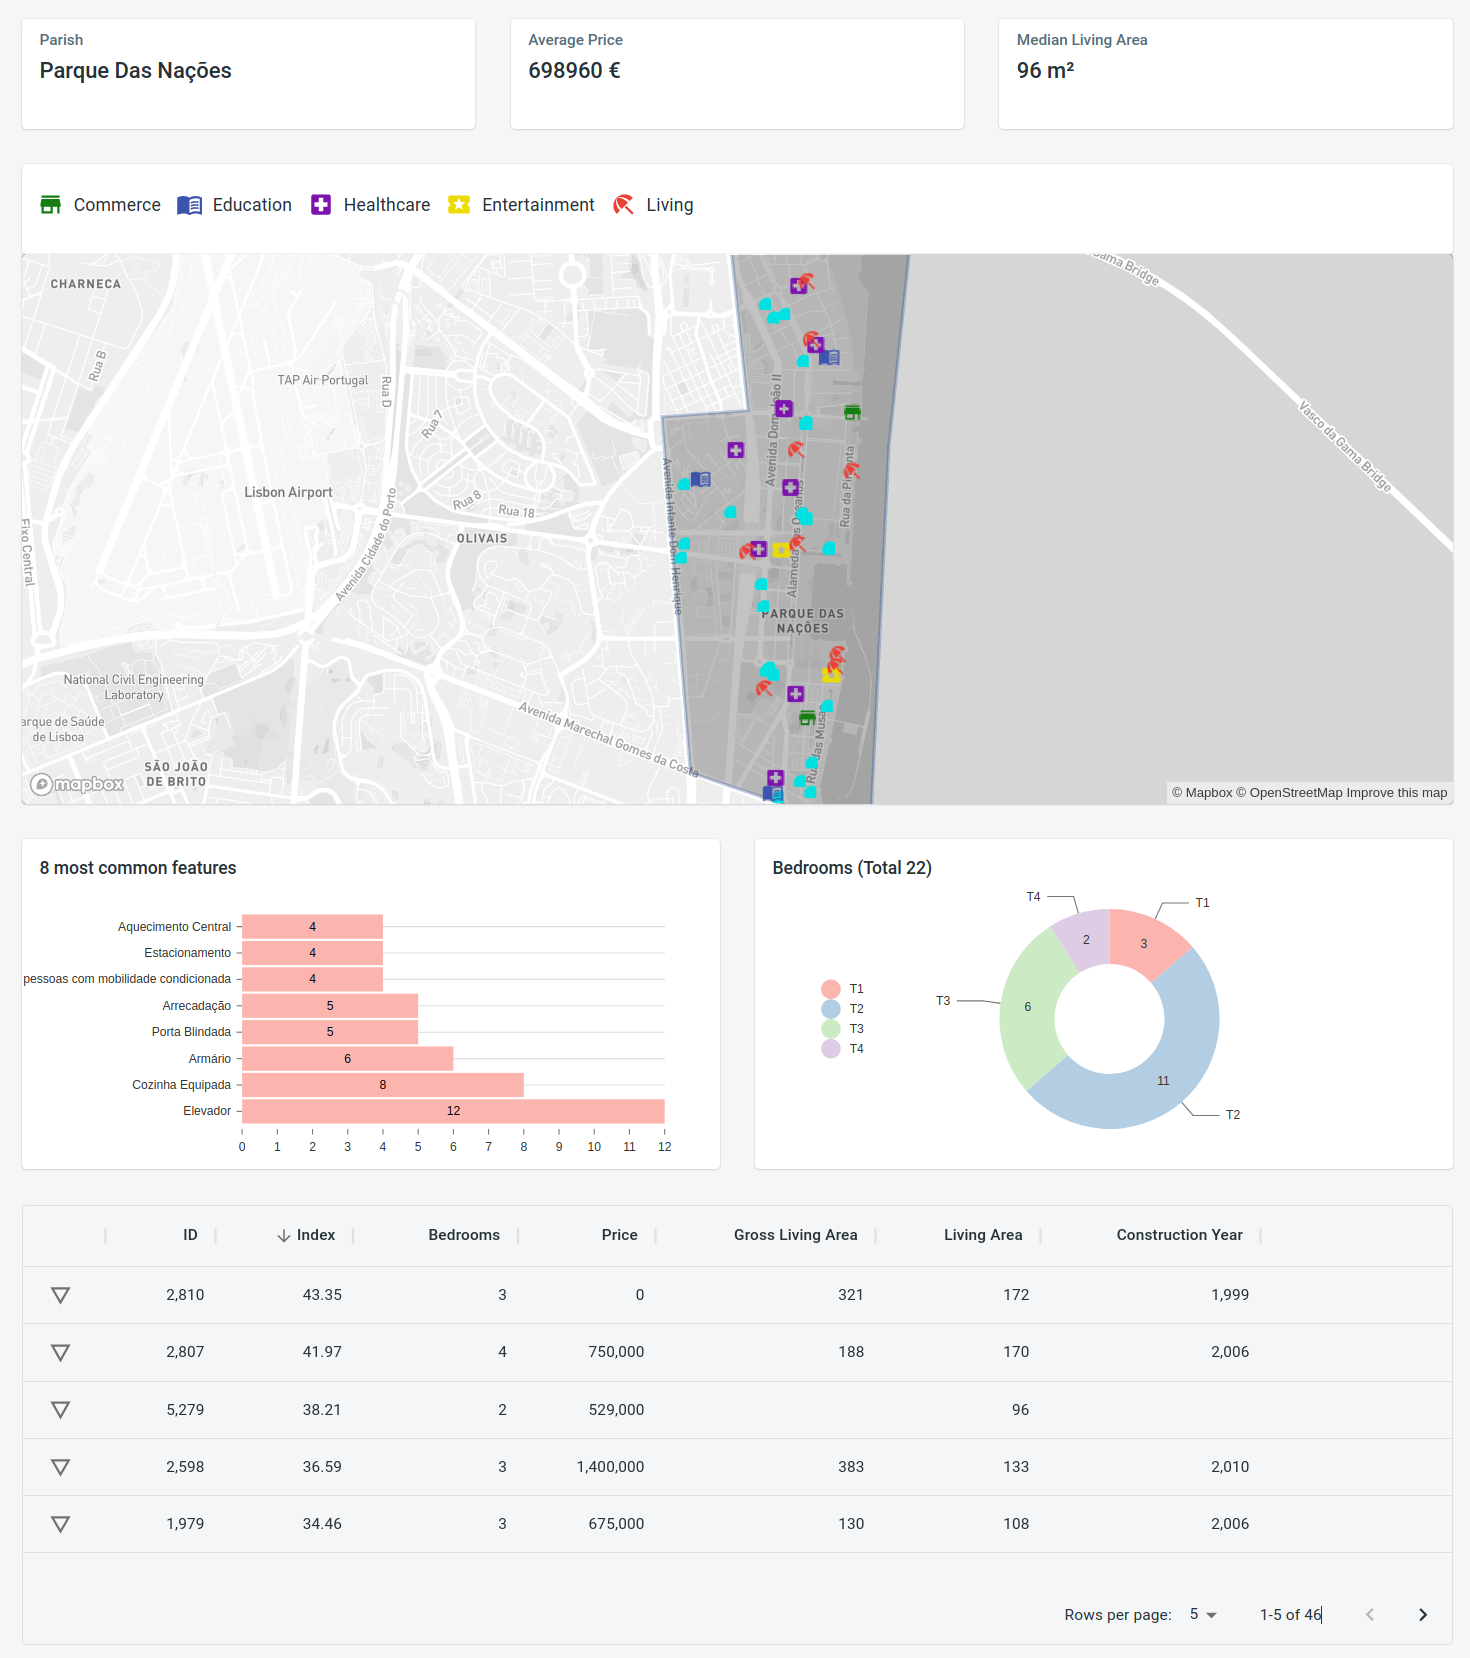
\includegraphics[width=1\textwidth,clip]{Chapters/img/frontend/Overview.png}};
        \node[xshift=-8cm, yshift= 8cm, fill=white, circle, draw=gray]{1)};
        \node[xshift=-8cm, yshift= 4cm, fill=white, circle, draw=gray]{2)};
        \node[xshift=-8cm, yshift=-2cm, fill=white, circle, draw=gray]{3)};
        \node[xshift=-8cm, yshift=-6cm, fill=white, circle, draw=gray]{4)};
    \end{tikzpicture}
    \caption{Overview of the dashboard} 
    \label{fig:overviewDashboard}
\end{figure}

As most of the data in the system relies is geographical, most of the queries are also within the same domain, endpoints like '/parish/1/estates' rely in PostGIS SQL functions like ST\_Contains to intersect estate Point coordinates with zone Polygons. One example of this queries can be seen in listing \ref{lst:geoQueryEstates}.

\begin{lstlisting}[float, language=SQL, label={lst:geoQueryEstates}, caption={[Example of geographical sql query returning a GeoJSON]{Example of a geographical query used in the project that returns the results formatted into a GeoJSON}}, captionpos=t]
SELECT jsonb_build_object('type', 'FeatureCollection', 'features', jsonb_agg(features.feature)) 
FROM ( 
    SELECT jsonb_build_object('type', 'Feature', 'id', id_estate, 'geometry', ST_AsGeoJSON(coordinates)::jsonb, 'properties', to_jsonb(inputs) - 'id_estate' - 'coordinates') AS feature
	FROM (
	    SELECT DISTINCT 
            estate.id_estate, location.coordinates, estate.typology, estate.living_area, estate.gross_living_area, construction_year,
            (SELECT price_history.value FROM price_history WHERE price_history.id_estate = location.id_estate ORDER BY update_date DESC LIMIT 1),
            (SELECT jsonb_agg(id_feature) FROM estate_features WHERE estate_features.id_estate = estate.id_estate) as features
        FROM locationType 
        INNER JOIN location ON ST_Contains(ST_SimplifyPreserveTopology(locationType.shape, SIMPLIFY_RATIO), location.coordinates)
        INNER JOIN estate ON estate.id_estate = location.id_estate
        INNER JOIN price_history ON estate.id_estate = price_history.id_estate
        WHERE locationType.idByType.get(locationType) = locationId) 
	inputs) 
features;
\end{lstlisting}

Most of the geographical queries created were built to return a GeoJSON, as a way to ensure interoperability between all the services and the frontend. Also, some of them had to be optimized to improve the speed of the queries, which also can be seen in the previous example as the shape of location was transformed with ST\_SimplifyPreserveTopology, which simplifies the geometry by removing some of its vertex while maintaining its original structure. Most of the commonly used geometries were also indexed, to ensure a faster access.

\subsubsection{Parameter}
\label{sss:parameter}

One of the most important factors of 15-minute cities is the essential functions that every citizen must be able to perform within a 15-minute radius. For this reason, an exclusive microservice was dedicated to dealing with services and commodities which take part in each function, and that we call  \acrfull{poi}. As a case-study all of the \acrshort{poi} are located in the Lisbon municipality, obtained through Lisboa Aberta~\footnote{\url{http://lisboaaberta.cm-lisboa.pt/index.php/pt/}}, the open Lisbon open data platform. For each function, the following data was gathered:

\begin{itemize}
    \item \textbf{Home} -- another word for estate, it has a dedicated service detail in section \ref{sss:estate};
    %\item \textbf{Work} -- As it would be difficult to track every job location, and
    \item \textbf{Commerce} -- Markets~\footnote{\url{https://dados.gov.pt/pt/datasets/mercados/}};
    \item \textbf{Health care} -- Pharmacies~\footnote{\url{http://dados.cm-lisboa.pt/dataset/farmacias-e-parafarmacias}} and public hospitals~\footnote{\url{http://dados.cm-lisboa.pt/dataset/hospitais-publicos}};
    \item \textbf{Education} -- First cycle (years 1st-4th)~\footnote{\url{https://dados.gov.pt/en/datasets/escolas-publicas-1-ciclo/}}
    \item \textbf{Entertainment} -- Museums~\footnote{\url{https://geodados-cml.hub.arcgis.com/datasets/museus}} and Cinemas~\footnote{\url{https://geodados-cml.hub.arcgis.com/datasets/CML::cinemas/}}.
    \item \textbf{Living} -- Green spaces~\footnote{\url{https://geodados-cml.hub.arcgis.com/datasets/e65d5898bfb443c9b19df421d8341734_0/explore?location=38.743700\%2C-9.155562\%2C13.38}}
\end{itemize}

The \textit{working} social function, mentioned previously during the introduction of the concept, was excluded from our interpretation, as it would exclude most estates searches (e.g., most people cannot afford to live near their workplace) while also saving the trouble of dealing with extra personal information that the user may be hesitant to give.

Each \acrshort{poi} is identified by a category (e.g., Health care and Entertainment), a service (e.g., Hospitals and Museums), a location represented through coordinates and finally, optional metadata to enrich the description of each \acrshort{poi}. As the relevant data is structured and fits a predefined schema we chose to pick PostgreSQL as a datastore, with the data model shown in Fig. \ref{fig:ea-params}. The populate the database data is ingested through a Python script which processes every GeoJSON file gathered previously.

\begin{figure}[h]
    \centering
    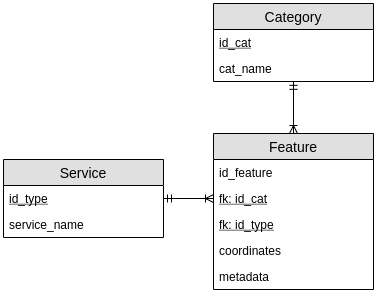
\includegraphics[width=0.5\textwidth,clip]{Chapters/img/backend/ea-params.png} 
    \caption{Parameter data model} 
    \label{fig:ea-params}
\end{figure}

When the user queries the system for a new zone, he is shown in the map where it is located while also being given the option to pick the categories he wishes to see in the map through toggling, as shown in Fig. \ref{fig:overviewMap}. 

\begin{figure}[h]
    \centering
    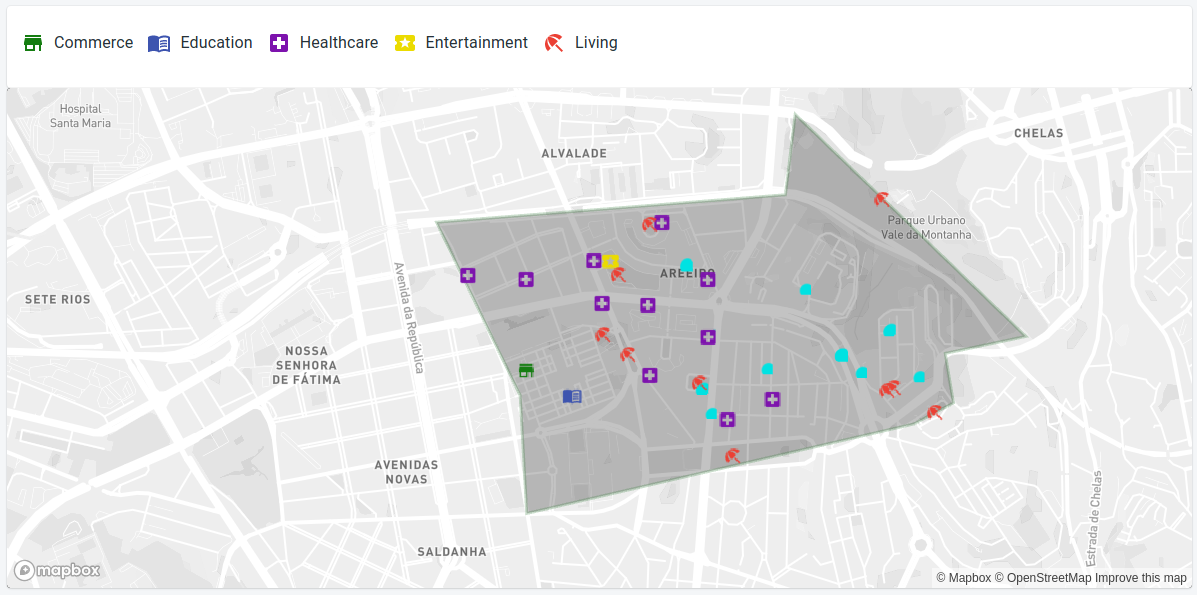
\includegraphics[width=1\textwidth]{Chapters/img/frontend/OverviewMap.png}
    \caption{Map as seen by the user} 
    \label{fig:overviewMap}
\end{figure}

All of this is supported through the following (Table \ref{tbl:paramsAPI}) endpoints available:

\begin{table}[h]
\centering
\begin{tabular}{c|c|c}
Type                     & Endpoint                                             & Description                                                                                                                                                    \\ \hline
GET                      & /features                                            & Retrieve all features with a geometry                                                                                                                          \\
GET                      & /feature/\{id\}                                      & Retrieve feature                                                                                                                                               \\
\multicolumn{1}{l|}{GET} & /category/\{id\}                                     & Retrieve category                                                                                                                                              \\
\multicolumn{1}{l|}{GET} & \multicolumn{1}{l|}{/estate/\{estate\_id\}/features} & \multicolumn{1}{l}{\begin{tabular}[c]{@{}l@{}}Retrieve features within isochrone geometry \\ surrouding the estate (depends on Metrics $\mu$ service)\end{tabular}}
\end{tabular}
\caption{/v1/params endpoints}
\label{tbl:paramsAPI}
\end{table}

\subsubsection{Search}

To facilitate site traversal a text-based search function was implemented with Elasticsearch. Through a search bar, the user is prompted to write the name of a location he wishes to look for, which can be any of the following types: parishes, municipalities, districts, and NUTS (1, 2 and 3). 

\begin{figure}[h]
    \centering
    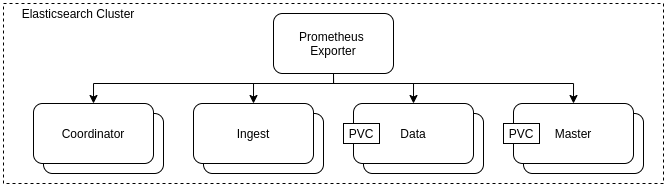
\includegraphics[width=1\textwidth]{Chapters/img/backend/es-architecture-sem-kibana.png}
    \caption{Elasticsearch cluster configuration} 
    \label{fig:es-architecture}
\end{figure}

The Elasticsearch cluster was deployed with the helm chart from Bitnami, and to maintain the goal of the rest of the entire application, it was adjusted to guarantee scalability by splitting the cluster into multiple nodes as seen in Fig. \ref{fig:es-architecture}. As of now, for the current workload, the application was deployed with only an instance of each node. The configuration was also setup to include a \textit{Prometheus exporter} node (details in section \ref{s:monitoring}), which is responsible for collecting metrics from each associated node, but as of now as it was not a top priority to monitor the Elasticsearch cluster, it remains unutilized.

The search functionality relies on location information acquired and used during the scraping phase, as such a Python script was created to ingest the data, but this time in the Elastic Search format, as shown in the following listing. 

\begin{lstlisting}[float, language=Python, caption={[Python data ingestion into Elastic Search]{Snippet of one the implementations done to insert data into the elastic search cluster with Python}}, captionpos=t]
def processDistrict(self, filepath, separator):
    # Colunas: 'Geo Point', 'Geo Shape', 'Dicofre', 'Distrito'
    # TIPOS:    String    ,  GeoJSON   ,  Int     ,  String

    df = pd.read_csv(filepath, sep=separator)

    actions = []
    for index, row in df.iterrows():
        action = {
            "_index": "locations-district",
            "_source": {
                "dist_district_name": row['Distrito'].title(),
                "dist_district_code": row['Dicofre'],
                "type": "District"
            }
        }
        actions.append(action)

    self.insertDataBulk(actions)
\end{lstlisting}

%in Python the same data was obtained from the database and inserted into Elasticsearch. 

%As this only occurs once during startup, and on rare occasions consequence of government updates, having a node dedicated to ingestion is a bit overkill, while at the same time facilitating future expansions.

The search bar was exposed to the frontend through a REST API (/v1/search) built in Spring Boot. It is split into five controllers, four of them for specific searches (e.g., /v1/search/district) and the last one, a generic controller used when the user has not specified the type of location he is looking for (/v1/search/location). For the latter, it has an associated \textit{LocationService} which is responsible for aggregating the data from all other services, allowing us to easily return results similar to the ones presented in Fig. \ref{fig:search-bar}.

\begin{figure}[h]
    \centering 
    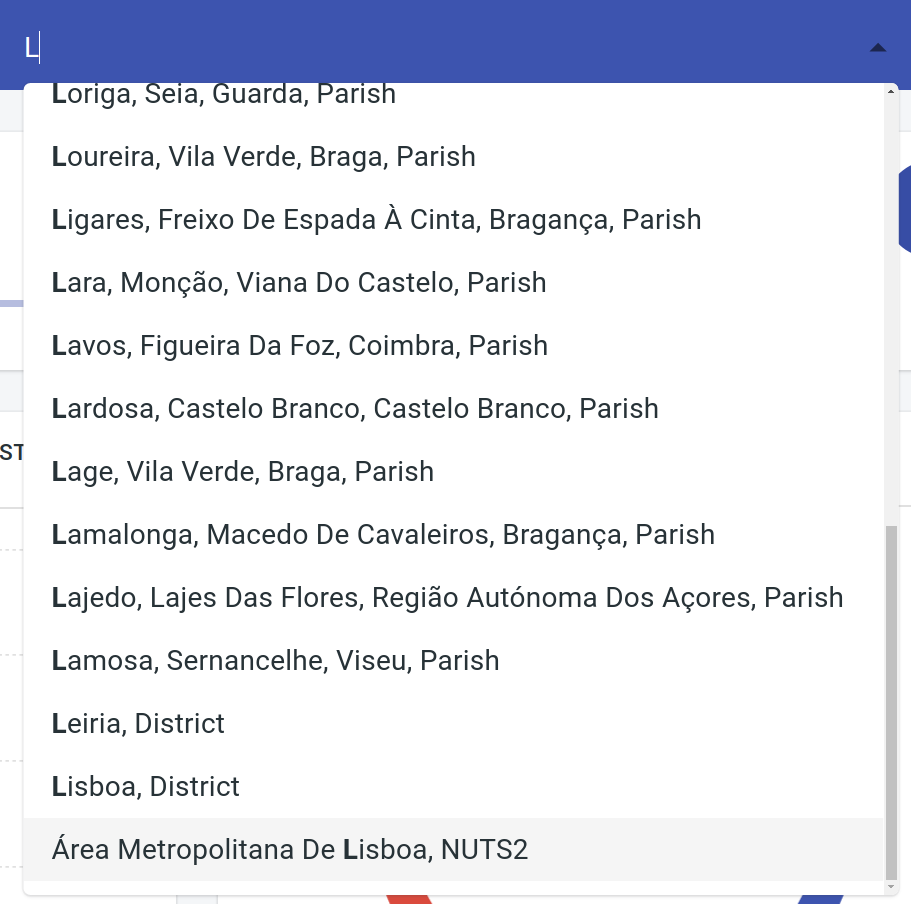
\includegraphics[width=0.4\textwidth]{Chapters/img/backend/search-bar.png}
    \caption{Search bar and results for the letter "L"} 
    \label{fig:search-bar}
\end{figure}

Each service has an associated repository that extends \textit{ElasticSearchRepository} from Spring Data, which works similarly to the repository described in Section \ref{sss:user} and allowed for generic querying of the cluster. However to be able to fine-tune the queries we had to implement a custom repository that each repository also extends, which uses the Elasticsearch full query \acrfull{dsl}. With this we were able to use existing queries such as: \textbf{Match phrase prefix query} which returns documents that contain the words of a provided text, in the same order as provided, with the last term being treated as a prefix, matching any words that begin with that term (e.g., "quick brown f" would match "quick brown fox" and "two quick brown ferrets" but not "the fox is quick and brown"); we also experimented with fuzzy queries, which return documents that contain terms similar to the search term (e.g, box--fox, black--lack, sic--sick, act--cat) but the results became inconsistent with more than two words, as fuzzy queries are term level queries Elasticsearch tries to search for entire phrases in lists of terms, which yields no results (e.g., "casal de cambra" would not find any match with the terms "casal", "de", "cambra" as there is no entry in the index for the whole phrase). 

\begin{figure}[h]
    \centering 
    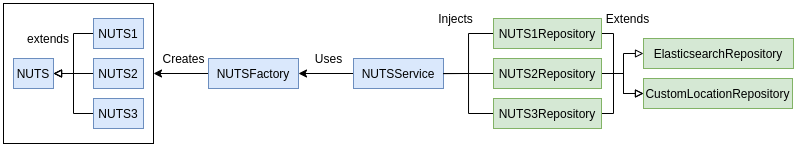
\includegraphics[width=1\textwidth]{Chapters/img/backend/nuts-es-horizontal.png}
    \caption{NUTS Factory pattern} 
    \label{fig:nuts-factory-pattern}
\end{figure}

\acrshort{nuts} are split into three different types, and to avoid creating three different services for each one, we decided to utilize the factory design pattern, as shown in Fig. \ref{fig:nuts-factory-pattern}. The \textit{NUTSService} now interacts solely with the NUTSFactory, and all its functions have a return type of the parent, NUTS. However, when fetching NUTS through the custom repository created and mentioned previously, Elasticsearch \acrshort{api} returns the results as \textit{SearchHits} instead of mapping them to the corresponding data models. To overcome this, we used reflection to determine the type of the instance and created the appropriate object, as seen in listing \ref{lst:nuts-reflection-snippet}. \\

\begin{lstlisting}[float, language = Java, caption={NUTS reflection snippet}, label={lst:nuts-reflection-snippet}, captionpos=t]
    String className = "microservice.search.model."+nutsType.getNutsType();
    Class[] cArg = {String.class,String.class, String.class, String.class};

    NUTS nut = (NUTS)Class
            .forName(className)
            .getDeclaredConstructor(cArg)
            .newInstance(id,regionName,regionCode,nutsType.getNutsType());
\end{lstlisting}

During the mapping of objects to their respective counterparts in the Elasticsearch cluster, text analysis had to be configured, which is the process of converting unstructured text, like the text fields in each object, into a structured format that's optimized for search. This configuration is done via a \acrshort{json} file and may be composed of three building blocks: character filters, tokenizers, and token filters.

\begin{itemize}
    \item \textbf{Character filters} receive the original text as a stream of characters and can transform the stream by adding, removing, or changing characters (e.g., converting hindu-arabic numerals to their arabic-latin equivalents).
    \item \textbf{Tokenizer} receives a stream of characters, breaks it up into individual tokens (words), and outputs a stream of tokens. For instance, a \textit{whitespace} tokenizer breaks text into tokens whenever it uses any whitespace. It is also responsible for recording the order or position of each term and the start and end character offsets of the original word which the term represents. An analyzer must always have one tokenizer. For our application, we chose the \textbf{edge\_ngram} tokenizer, a common tool for \textit{search-as-you-type} queries, which first breaks text down into words whenever it encounters one of a list of specified characters, then it emits \textit{\gls{n-gram}s} of each word where the start of the N-gram is anchored to the beginning of the word.  
    \item \textbf{Token filter} receives the token stream and may add, remove, or change tokens. For example, in our case it was configured to use the following filters: \textbf{lowercase} token filter converts all tokens to lowercase and \textbf{ASCII folding}, which converts alphabetic, numeric, and symbolic characters that are not in the Basic Latin Unicode block (first 127 characters) to their ASCII equivalent, if it exists (e.g., changing é to e).
\end{itemize}

The following endpoints (Table \ref{tbl:searchAPI}) are made available to the public, where \$type is used to simplify the table, in the code there's an endpoint for each of these scenarios for the multiple types of locations: NUTS, districts, municipalities, and parishes. 

\begin{table}[h]
\centering
\caption[Endpoints available in the search API]{Endpoints available in the search microservice at /v1/search.}
\begin{tabular}{c|c|c}
Type                     & Endpoint                                                & Description                                 \\ \hline
GET                      & /\$type (ex: /municipalities)                           & Retrieve all                                \\
GET                      & /\$type/\{name:\textasciicircum{}{[}A-zÀ-ú{]}\{1,27\}\} & Retrieve by name, validated through regex   \\
\multicolumn{1}{l|}{GET} & /\$type/\{code\}                                        & Retrieve by code                            \\
\multicolumn{1}{l|}{GET} & /locations                                              & Searchs all types at the same time, by name
\end{tabular}

\label{tbl:searchAPI}
\end{table}


\subsubsection{Metrics}
\label{sss:metrics}


To enrich the user experience, and truly bring to life the 15 minute concept, it was important to display relevant information about each zone pertaining the containing estates. The metrics microservice requires information scattered through out all the services and as such, it required an efficient way to communicate. 

The metrics that depend solely on estates (Median price, median square metre, most common features and typology distribution) are all requested simultaneously to the estate service through Kafka. The information is request synchronously, something Kafka is not usually associated with. To achieve the request-reply pattern, a correlation ID is associated with each record, allowing Kafka to identify each transaction and correlate requests/replies. As of version 2.1.3, Spring Kafka added support for the Request Reply pattern out-of-the-box which abstracts some of the previous concepts.

\begin{figure}[h]
    \centering 
    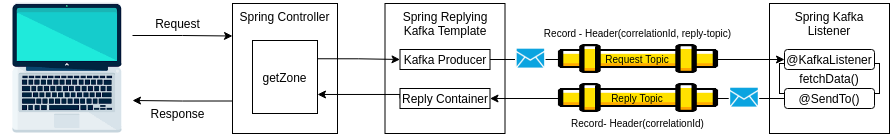
\includegraphics[width=1\textwidth]{Chapters/img/backend/KafkaReqReply.png}
    \caption{Synchronous Request-Reply with Apache Kafka} 
    \label{fig:ReqRepKafka}
\end{figure}

As seen in Fig. \ref{fig:ReqRepKafka}, the user sends a request to the controller asking for information about the zone. The endpoint utilizes the \textbf{kafka reply template} to create a message which includes all the necessary header information such as the \textit{correlation id}, additional information such as \textit{zone id} and the \textit{reply topic} it expects to hear a response from, are manually configured. 

In the other microservice, a \textbf{Kafka Listener} was implemented which is actively waiting for messages, the method is also annotated with \textbf{SendTo} to provide a reply message. The object returns by the listener is automatically wrapped into a reply message, the \textit{correlation id}, and the reply is sent to the specified \textit{reply topic}, which eventually is return to the user.

Since estate data is scrapped and stored every 7 days, there always the guarantee that whatever was fetched up to that day is guaranteed fresh as such, to avoid wasting time and resources of having to constantly communicate with other microservices, data is stored in a MongoDB node associated with this microservice. In every request to \textbf{getZone} (Fig. \ref{fig:ReqRepKafka}), we verify if the data is fresh based on the date it was gathered, and if it is, we can simply query the database and answer the request instantly.


%% ===================================================== Index =============================================================================
\paragraph{Index} is used to rate an estate according to the users social and real estate preferences. To calculate this rating, a weight was associated with each choice. 

As the concept accounts for five main social functions, each had an associated weight that started at 30 and would decrease in steps of 5 (e.g., 30, 25, 20, 15, and 10), associating 30 with the users first option and 10 with the last. Associated to each social function, there are multiple services, which at the moment are averaged down and considered as one, but can easily in the future be altered to account for each specific service. The previous idea can be translated into the following equation:

\begin{equation}
    SocialIndex = \sum_{sf = social\_function} sf \ weight(\%) * max(1, Avg(\frac{ideal\_distance }{dist<estate,service>})
\end{equation}

The ideal distance was considered based on the idea that within a 5 minute window everything is still close enough. As the distance varies according to the chosen travel mode, three values were chosen for each of them, as depicted in Table \ref{tbl:idealTravelDistance}.

\begin{table}[h]
\centering
\caption{[Ideal travel distance in the 15-Minute City per travel mode]{Our idealized travel distance values. Within this range, it is considered that it is not an annoyance to travel somewhere}}
\begin{tabular}{c|c}
Travel Mode & Distance (m) \\ \hline
walking     & 400          \\
cycling     & 1300         \\
driving     & 3000        
\end{tabular}

\label{tbl:idealTravelDistance}
\end{table}


For estate features, since the user can select between 1 and 5 options, the weights are calculated based on the number of options (e.g., $\frac{number \ of \ features}{features \ weight \ \%}$ ), so the feature index arises from the following formula

\begin{equation}
    FeatureIndex = \frac{features \ weight \ \%}{\#user\_selected\_features} * \#relevant\_features
\end{equation}

Both sections are then combined to create the \textbf{index} that always yields results between 0 and 100\%:

\begin{equation}
    Index = (SocialIndex * SocialWeight) + FeatureIndex
\end{equation}

As mentioned previously, and as seen through the equation, to calculate the index, it requires information from multiple points of the system and even external APIs:

\begin{itemize}
    \item \textbf{User} information such as favorite features, social preferences, travel mode;
    \item \textbf{Location} retrieving the GeoJSON from the selected zone;
    \item \textbf{Estates} obtain a list of estates from the selected zone;
    \item \textbf{Parameters} list of points of interest surrounding the estates;
    \item \textbf{Isochrone} map depicts the area accessible from a point within a certain time treshold, information which was gathered from the Mapbox API \footnote{\url{https://docs.mapbox.com/api/navigation/isochrone/}}.
\end{itemize}

Fig. \ref{fig:IndexSequenceDiagram} shows the sequence of actions made to calculate the index, the main idea is that when a user requests a new zone, all the estates in that specific area are fetched, if they already have an associated isochrone for the specified travel model it is used to calculate the index, otherwise a request is made to the mapbox \acrshort{api} to calculate it and store it.

\begin{figure}[h]
    \centering 
    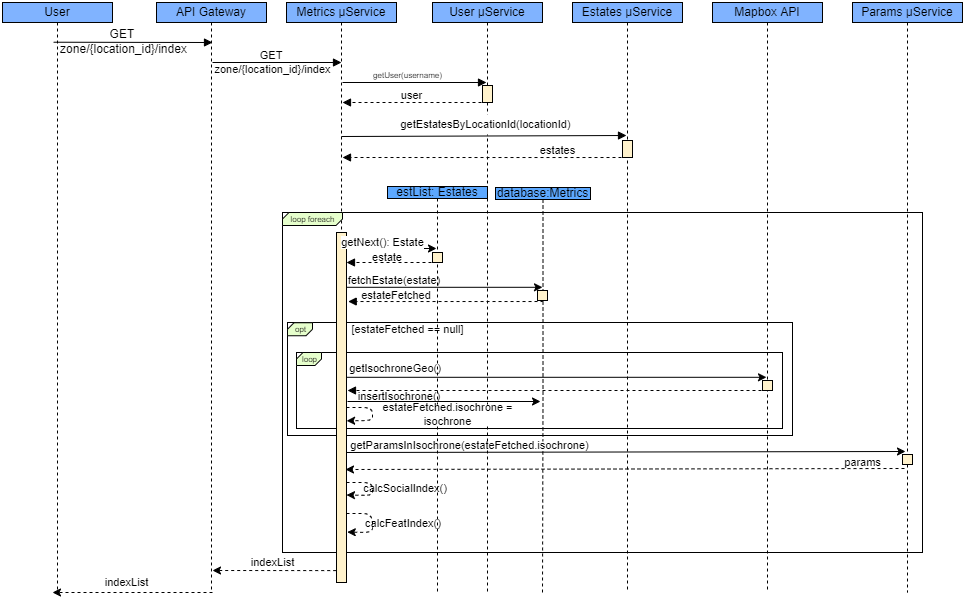
\includegraphics[width=1\textwidth]{Chapters/img/backend/SequenceDiagram.png}
    \caption{Index calculation sequence diagram} 
    \label{fig:IndexSequenceDiagram}
\end{figure}

Unlike the previous case which used Kafka as an intermediary to communicate between services, the index calculation only uses \textbf{gRPC} to interact with all the services. For this interaction a stub was defined for each microservices in the client side (metrics microservice) and a gRPC server in the respective microservices. To communicate a \textit{.proto} file had to be created, to define the services and messages required to communicate. A particularity of this definition its that User is composed by two submessages, similar to OOP concepts, where in this case \textit{features} and \textit{services} have their own definitions to mimic lists.

\begin{lstlisting}[float, language=Java, caption={[GRPC message and service definitions]{GRPC message and service definitions for communication}}, captionpos=t]
syntax = "proto3";
option java_multiple_files = true;
package demo.interfaces.grpc;

message User{
  message ListFeatures{
    repeated int32 feature = 1;
  }

  message ListServices{
    repeated int32 services = 1;
  }

  string id = 1;
  string username = 2;
  ListFeatures features = 3;
  ListServices services = 4;
  int32 surroundingsPercentagePreference = 5;
  int32 estateFeaturesPercentagePreference = 6;
  string travelModel = 7;
}

message Username{
  string username = 1;
}

service UserService {
  rpc getUserByUsername(Username) returns (User);
}
\end{lstlisting}

To obtain the corresponding data access classes and services, the proto file had to be compiled, isntead of doing it manually the process was automatized with Maven and \textit{Maven Protocol Buffers Plugin}~\footnote{\url{https://www.xolstice.org/protobuf-maven-plugin/}}. After the compiler creates the \textit{.java} files for each message type and service, it is now possible to implement the client and server stubs, which can be seen in the following listings.

\begin{lstlisting}[float, language=Java, caption={Java service for GRPC communication}, captionpos=t]
@Service
public class UserServiceImpl{
    @GrpcClient("user-service") 
    private UserServiceBlockingStub userServiceBlockingStub;

    public User getUserByUsername(String username){
        Username request = Username.newBuilder().setUsername(username).build();
        demo.interfaces.grpc.User user;
        try{ user = userServiceBlockingStub.getUserByUsername(request);
        } catch (StatusRuntimeException e){ return null; }
        return new User(user);
    }
}
\end{lstlisting}

The main advantage with gRPC is that there is no need to handle the serialization and deserialization of the transmitted objects, especially when using the same language on both the server and client. When the proto file was compiled the \textbf{UserServiceImplBase} was created, which can be used on the server with an implementation for the defined services, which can then be called by the client as remote procedure calls.

\begin{lstlisting}[float, language=Java, caption={Service definition}, captionpos=t]
@GrpcService
public class UserServiceImpl extends UserServiceGrpc.UserServiceImplBase {
    @Autowired private DynamoService dynamoService;
    @Override 
    public void getUserByUsername(Username request, StreamObserver<User> responseObserver){
        String username = request.getUsername();
        UserDynamo user = dynamoService.getUserByUsername(username);

        ListFeatures.Builder listFeaturesBuilder = ListFeatures
                .newBuilder()
                .addAllFeature(user.getFeaturePreferences()
                                .stream()
                                .map(Integer::parseInt)
                                .collect(Collectors.toList()));

        ListServices.Builder listServicesBuilder = ListServices
                                .newBuilder()
                                .addAllServices(user.getServicePreferences());

        User.Builder userBuilder = User.newBuilder()
                .setId(user.getId())
                .setUsername(user.getUsername())
                .setFeatures(listFeaturesBuilder.build())
                .setServices(listServicesBuilder.build())
                .setSurroundingsPercentagePreference(user.getSurroundingsPercentagePreferences())
                .setEstateFeaturesPercentagePreference(user.getEstateFeaturesPercentagePreferences())
                .setTravelModel(user.getTravelMode());

        responseObserver.onNext(userBuilder.build());
        responseObserver.onCompleted();
    }
}
\end{lstlisting}

The following endpoints (Table \ref{tbl:metricsAPI}) are available to the public.


\begin{table}[h]
\centering
\begin{tabular}{c|c|c}
Type                     & Endpoint                                          & Description                                                                                                              \\ \hline
GET                      & /estate/\{estate\_id\}/isochrone/\{travel\_mode\} & \begin{tabular}[c]{@{}c@{}}Retrieve estate isochrone geometry \\ based on travel mode\end{tabular}                       \\
GET                      & /estate/\{estate\_id\}/params                     & \begin{tabular}[c]{@{}c@{}}Retrieve params inside an estate \\ (uses Params $\mu$service)\end{tabular}                       \\
\multicolumn{1}{l|}{GET} & /zone/\{location\_id\}/index                      & \begin{tabular}[c]{@{}c@{}}Calculates the index for the estates \\ in a zone,  to the user who requested it\end{tabular} \\
\multicolumn{1}{l|}{GET} & /zone/\{location\_id\}                            & \begin{tabular}[c]{@{}c@{}}Retrieves/Calculates metrics \\ for the specific zone\end{tabular}                                                                   
\end{tabular}
\caption{Endpoints available at /v1/metrics}
\label{tbl:metricsAPI}
\end{table}

With access to all of this information, the frontend is capable of presenting to the user the metrics shown in Fig. \ref{fig:overviewMetrics}.

\begin{figure}[h]
    \centering 
    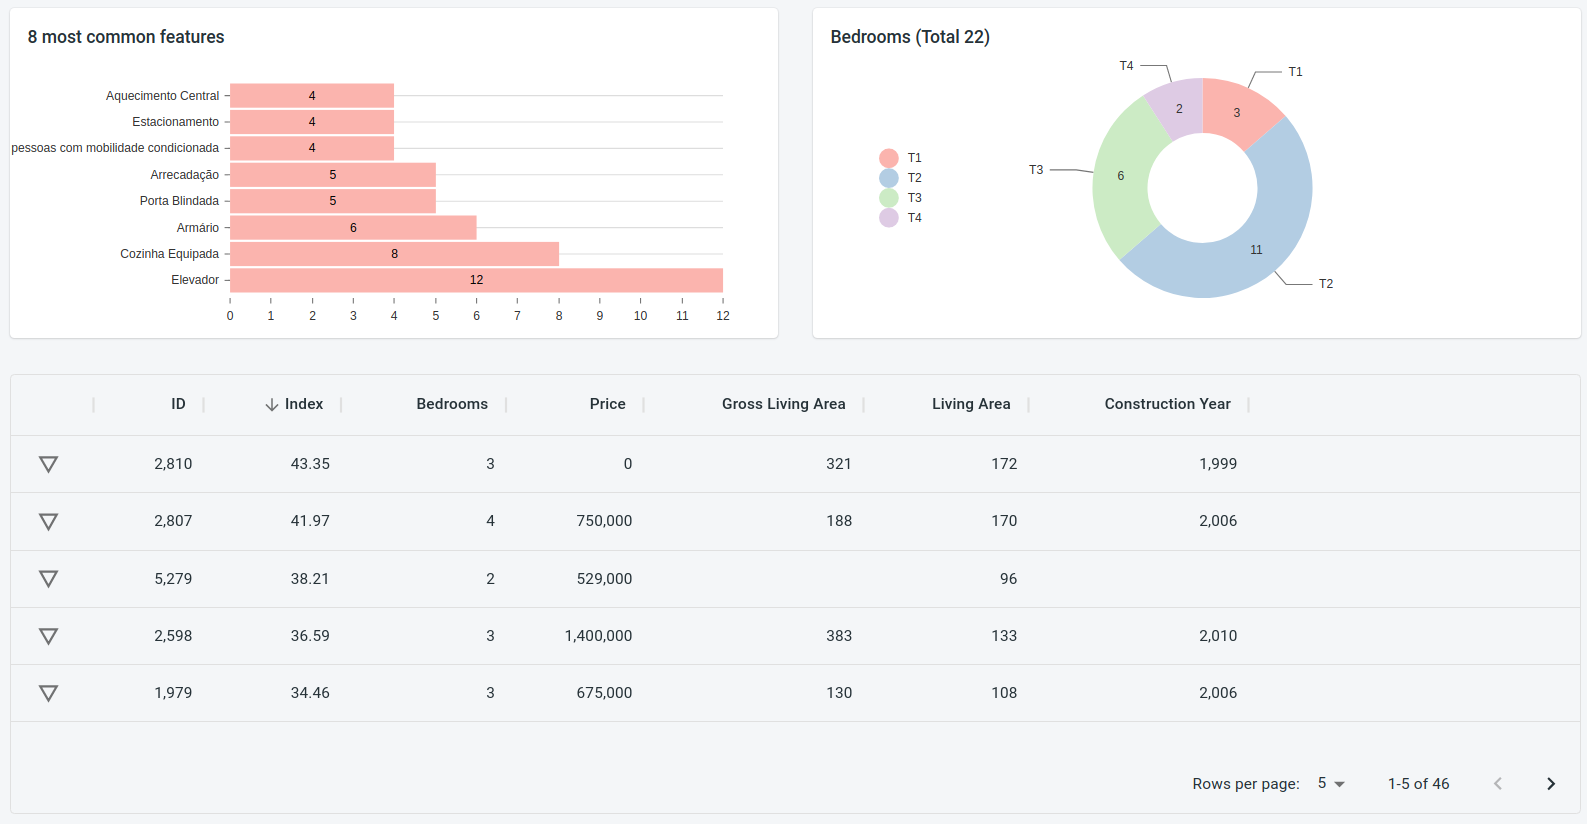
\includegraphics[width=1\textwidth]{Chapters/img/frontend/OverviewMetrics.png}
    \caption{Dashboard - metrics section} 
    \label{fig:overviewMetrics}
\end{figure}



